\documentclass[]{standalone}
\usepackage{amsmath,amssymb}
%matrix
\newcommand{\mt}[1]{\ensuremath{\mathbf{#1}}}
%vector
\newcommand{\vc}[1]{\ensuremath{\boldsymbol{#1}}}
%set
\newcommand{\st}[1]{\ensuremath{\mathcal{#1}}}
%time index
\newcommand{\tm}[1]{\ensuremath{\sp{(#1)}}}


%x
\newcommand{\x}[0]{\ensuremath{\vc{x}}}
%s
\newcommand{\s}[0]{\ensuremath{\vc{s}}}
%W
\newcommand{\W}[0]{\ensuremath{\mt{W}}}



\usepackage{pgf}
\usepackage{tikz}
\usetikzlibrary{arrows,automata,matrix}
\usepackage[latin1]{inputenc}
\begin{document}
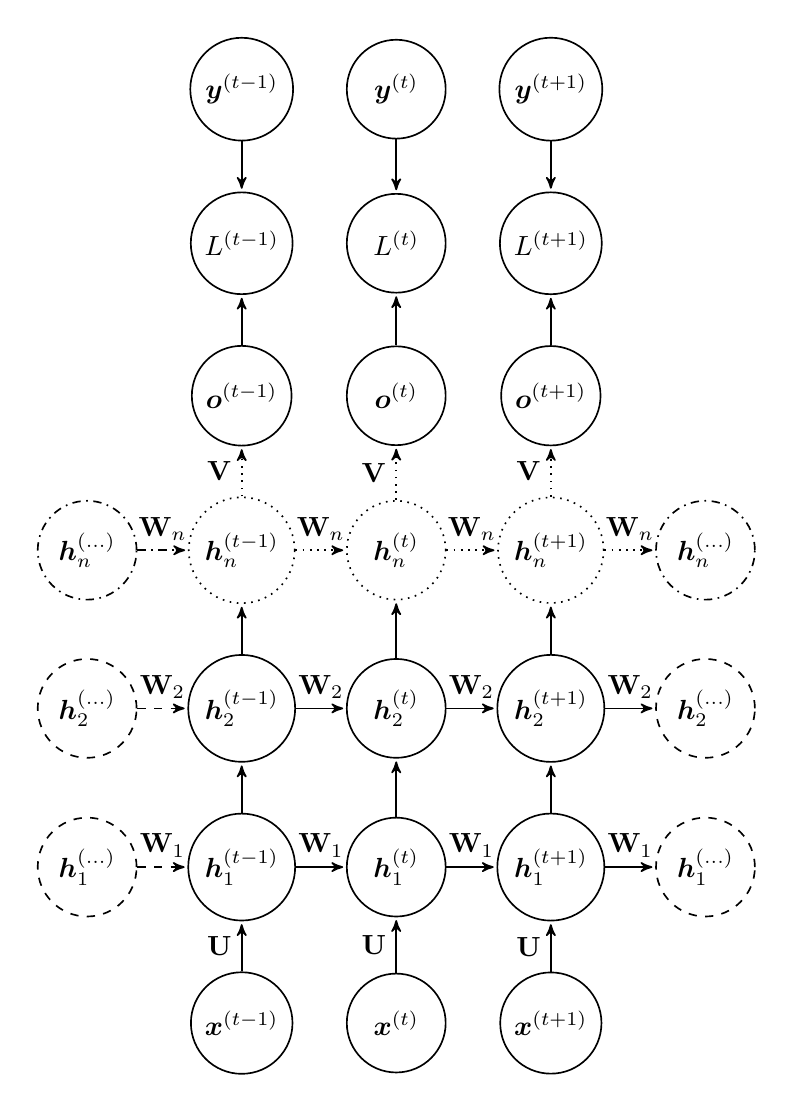
\begin{tikzpicture}[->,>=stealth'
	,shorten >=1pt
	,auto
	,node distance=2.8cm,
              semithick]
  \tikzstyle{every state}
  =[minimum size={10pt+width("$x^{(t-1)}$")}]

  \matrix (m) [matrix of nodes
  ,row sep=.25in,column sep=.25in] {
    % 3 ys
    &
    \node[state](ytm1) {$\vc{y}^{(t-1)}$}; &
    \node[state](yt) {$\vc{y}^{(t)}$};    &
    \node[state](ytp1) {$\vc{y}^{(t+1)}$}; 
    \\
    % 3 Ls
    &
    \node[state](Ltm1) {$L^{(t-1)}$}; &
    \node[state](Lt) {$L^{(t)}$}; &
    \node[state](Ltp1) {$L^{(t+1)}$};
    \\
    % 3 os
    &
    \node[state](otm1) {$\vc{o}^{(t-1)}$}; &
    \node[state](ot) {$\vc{o}^{(t)}$}; &
    \node[state](otp1) {$\vc{o}^{(t+1)}$};
    \\
    % 5 hns
    \node[state,dashdotted](hndm) {$\vc{h}_n^{(\ldots)}$}; &
    \node[state,dotted](hntm1) {$\vc{h}_n^{(t-1)}$}; &
    \node[state,dotted](hnt) {$\vc{h}_n^{(t)}$}; &
    \node[state,dotted](hntp1) {$\vc{h}_n^{(t+1)}$}; &
    \node[state,dashdotted](hndp) {$\vc{h}_n^{(\ldots)}$};
    \\
    % 5 h2s
    \node[state,dashed](h2dm) {$\vc{h}_2^{(\ldots)}$}; &
    \node[state](h2tm1) {$\vc{h}_2^{(t-1)}$}; &
    \node[state](h2t) {$\vc{h}_2^{(t)}$}; &
    \node[state](h2tp1) {$\vc{h}_2^{(t+1)}$}; &
    \node[state,dashed](h2dp) {$\vc{h}_2^{(\ldots)}$};
    \\
    % 5 h1s
    \node[state,dashed](h1dm) {$\vc{h}_1^{(\ldots)}$}; &
    \node[state](h1tm1) {$\vc{h}_1^{(t-1)}$}; &
    \node[state](h1t) {$\vc{h}_1^{(t)}$}; &
    \node[state](h1tp1) {$\vc{h}_1^{(t+1)}$}; &
    \node[state,dashed](h1dp) {$\vc{h}_1^{(\ldots)}$}; 
    \\
    % 3 xs
    &
    \node[state](xtm1) {$\vc{x}^{(t-1)}$}; &
    \node[state](xt) {$\vc{x}^{(t)}$};    &
    \node[state](xtp1) {$\vc{x}^{(t+1)}$};
    \\
  };
  % left to right, top to bottom.
  % each layer outgoing and within itself arrows
  % minus ... 
  \path [dashdotted] (hndm)  edge  node {$\mt{W}_n$} (hntm1);
  \path [dashed] (h2dm)  edge  node {$\mt{W}_2$} (h2tm1);
  \path [dashed] (h1dm)  edge  node {$\mt{W}_1$} (h1tm1);
  % t-1
  \path [      ] (ytm1)  edge  node {     }      (Ltm1);
  \path [      ] (otm1)  edge  node {     }      (Ltm1);
  \path [dotted] (hntm1) edge  node {$\mt{V}$}   (otm1);
  \path [      ] (h2tm1) edge  node {}           (hntm1);
  \path [      ] (h1tm1) edge  node {}           (h2tm1);
  \path [      ] (xtm1)  edge  node {$\mt{U}$}   (h1tm1);
  \path [dotted] (hntm1) edge  node {$\mt{W}_n$} (hnt);
  \path [      ] (h2tm1) edge  node {$\mt{W}_2$} (h2t);
  \path [      ] (h1tm1) edge  node {$\mt{W}_1$} (h1t);
  % t
  \path [      ] (yt)    edge  node {     }      (Lt);
  \path [      ] (ot)    edge  node {     }      (Lt);
  \path [dotted] (hnt)   edge  node {$\mt{V}$}   (ot);
  \path [      ] (h2t)   edge  node {}           (hnt);
  \path [      ] (h1t)   edge  node {}           (h2t);
  \path [      ] (xt)    edge  node {$\mt{U}$}   (h1t);
  \path [dotted] (hnt)   edge  node {$\mt{W}_n$} (hntp1);
  \path [      ] (h2t)   edge  node {$\mt{W}_2$} (h2tp1);
  \path [      ] (h1t)   edge  node {$\mt{W}_1$} (h1tp1);
  % t+1
  \path [      ] (ytp1)  edge  node {     }      (Ltp1);
  \path [      ] (otp1)  edge  node {     }      (Ltp1);
  \path [dotted] (hntp1) edge  node {$\mt{V}$}   (otp1);
  \path [      ] (h2tp1) edge  node {}           (hntp1);
  \path [      ] (h1tp1) edge  node {}           (h2tp1);
  \path [      ] (xtp1)  edge  node {$\mt{U}$}   (h1tp1);
  % plus ...
  \path [dotted] (hntp1) edge  node {$\mt{W}_n$} (hndp);
  \path [      ] (h2tp1) edge  node {$\mt{W}_2$} (h2dp);
  \path [      ] (h1tp1) edge  node {$\mt{W}_1$} (h1dp);

  
\end{tikzpicture}

\end{document}